\documentclass{article}
\usepackage{tikz}
\usepackage{amsmath}
\usepackage[a4paper]{geometry}
\usepackage{fancyhdr}
\pagestyle{fancy}
\lhead{Geometrische Figuren im Raum}
\rhead{August 2025}
\begin{document}
  
\newcommand{\normp}[1]{\big| \vectp{#1} \big|}  
\newcommand{\norm}[1]{\big| {#1} \big|}  
\newcommand{\vectp}[1]{\vect{\mathrm{#1}}}
\newcommand{\vect}[1]{\overrightarrow{#1}} 
 
\section{Geometrische Figuren im Raum} 
\begin{minipage}{\dimexpr\linewidth-5cm}
 Mehrere Punkte können zusammen eine geometrische Figur ergeben. Die Verbindungsvektoren zwischen den Punkten stellen dabei die Linien zwischen den Punkten dar, sodass die Beträge der Vektoren die Länge der Linien darstellen. \newline
 Anhand dieser Vektoren kann die Länge und Richtung der Seiten und die Winkelgrößen der Winkel gefunden werden. \newline
 Mit diesen können alle bereits bekannten Formeln und Regeln zu geometrische Figuren im Raum angewand werden, nur das hier die Seitenlängen die Vektorenbeträge sind. So wie Formel für das Volumen eines Quaders $V = a \cdot b \cdot c$ ist, die $\text{Länge} \times \text{Breite} \times \text{Höhe}$ sind diese hier $V = \normp{AB} \cdot \normp{AC} \cdot \normp{AD}$. Durch das Vergleichen der Seitenlängen und den Winkeln kann auch nachgewiesen werden, dass eine Figur tatsächlich ein Quader oder ein Würfel oder ähnliches ist.
\end{minipage}
\hfill
\begin{minipage}{5cm}
 \center 
 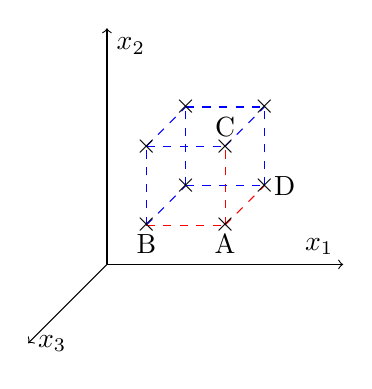
\begin{tikzpicture}  
  \draw[->] (0, 0) -- (3, 0) node [above left] {$x_1$}; 
  \draw[->] (0, 0) -- (0, 3) node [below right] {$x_2$};
  \draw[->] (0, 0) -- (-1, -1) node [right] {$x_3$};
  
  \draw[red, dashed] (0.5, 0.5) -- (1.5, 0.5);
  \draw[blue, dashed] (0.5, 1.5) -- (1.5, 1.5);
  \draw[blue, dashed] (0.5, 0.5) -- (0.5, 1.5);
  \draw[red, dashed] (1.5, 0.5) -- (1.5, 1.5);
 
  \draw[blue, dashed] (1, 1) -- (2, 1);
  \draw[blue, dashed] (1, 2) -- (2, 2);
  \draw[blue, dashed] (1, 1) -- (1, 2);
  \draw[blue, dashed] (2, 1) -- (2, 2);
 
  \draw[blue, dashed] (0.5, 0.5) -- (1, 1);
  \draw[blue, dashed] (0.5, 1.5) -- (1, 2);
  \draw[red, dashed] (1.5, 0.5) -- (2, 1);
  \draw[blue, dashed] (1.5, 1.5) -- (2, 2); 
  \draw (0.5, 0.5) node {$\times$} node [below] {B};
  \draw (1.5, 0.5) node {$\times$} node [below] {A};
  \draw (0.5, 1.5) node {$\times$};
  \draw (1.5, 1.5) node {$\times$} node [above] {C};
  
  \draw (1, 1) node {$\times$};
  \draw (2, 1) node {$\times$} node [right] {D};
  \draw (1, 2) node {$\times$};
  \draw (2, 2) node {$\times$};
 \end{tikzpicture}   
\end{minipage} 
 
 
\end{document}
 
